Dieses Kapitel soll dem späteren Bediener des Versuchstand die Handhabung vereinfachen und auf potenzielle Fehlerquellen sowie Gefahren hinweisen.



\section{Quick Start Guide}
Dieses Kapitel gibt einen schnellen Überblick darüber wie der Versuchstand zu bedienen ist. 
\begin{figure}[!h]
    \centering
    \begin{subfigure}[]{.45\textwidth}
        \centering
        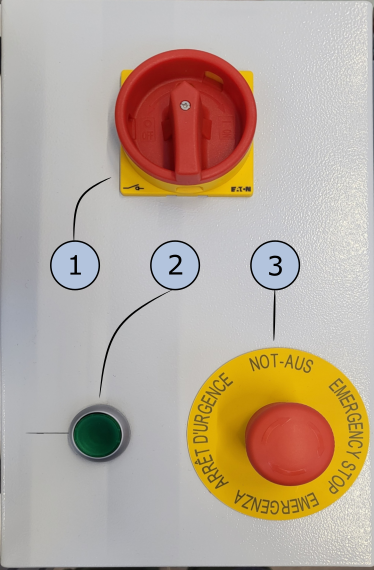
\includegraphics[width=0.8\textwidth]{Abbildungen/Manuel/Schrank_oben_bb_oo.png}
        
    \end{subfigure}
    \begin{subfigure}[]{.45\textwidth}
            \begin{tabular}{c|l}
               1    & Hauptschalter\\
               2    & EIN Taster  \\
               3    & NOT-AUS Schalter
            \end{tabular}
    \end{subfigure}
    \caption{Oberseite Schaltschrank}
    \label{fig:b_schaltschrank}   
\end{figure}

Vor Inbetriebnahme sollte immer geprüft werden ob Irgentwelche Teile der Mechanik durch Fremdeinwirkung blockiert sind. Ist dies nicht der Fall kann der Schuko-Stecker in die Steckdose gesteckt werden. In Abbildung \ref{fig:schaltschrank} ist die Oberseite des Schaltschrankes zu sehen, mit welcher die Anlage eingeschaltet werden kann. Nun kann durch drehen des Hauptschalters (1) im Uhrzeigersinn  die Anlage unter Spannung gesetzt werden. Mittels Taster (2) wird sowohl die Lastspannung für die Motoren als auch die Spannung für das Bedienfeld sowie den Temperaturregler der Heizung Eingeschaltet. Zum Ausschalten der Apperatur den Hauptschalter (1) gegen den Uhrzeigersinn drehen. Der NOT-AUS Schalter (3) schaltet den Versuchstand ebenfalls ab und verhindert zusätzlich ein wiedereinschalten.
\newpage
\begin{figure}[!h]
    \centering
    \begin{subfigure}[]{.45\textwidth}
        \centering
        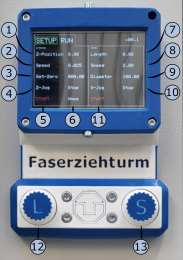
\includegraphics[width=0.8\textwidth]{Abbildungen/Manuel/Interface_01.png}
        \caption{Interface}
        \label{fig:interface}
    \end{subfigure}
    \begin{subfigure}[]{.45\textwidth}
        \centering
        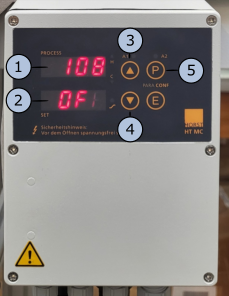
\includegraphics[width=0.88\textwidth]{Abbildungen/Manuel/Interface_02.png}
        \caption{HTMC}
        \label{fig:HTMC}
    \end{subfigure}
    \begin{subfigure}[]{.45\textwidth}
        \centering
        \begin{tabular}{c|l}
        
               12    & Wahlrad Z-Achse \\
               13    & Wahlrad Abzug 
        \label{tab:interface}     
        \end{tabular}
        
        
    \end{subfigure}
    \begin{subfigure}[]{.45\textwidth}
    \centering
        \begin{tabular}{c|l}
               3    & Temperatursollwert erhöhen\\
               4    & Temperatursollwert verringern \\
               5    & Sollwert setzten
            
        \label{tab:HTMC}      
        \end{tabular}
        
    \end{subfigure}
    \caption{Bedienfelder des Versuchstandes}
    \label{fig:bedienfelder}  
\end{figure}

Für die Steuerung der Motoren ist das in Abbildung \ref{fig:interface} datgestellte Bedienfeld verantwortlich. Zu beginn sollte die Z-Achse in ihre Ausgangsposition gefahren werden. Dazu einfach durch drehen des Wahlrads (12) zum Menüpunkt (6) navigieren und durch drücken des Rades bestätigen. Nun sollte die Linearachse zum oberen Endanschlag fahren. Als nächste können alle gewünschten Betriebseinstellungen verändert werden. Das Verändern eines Parameters funktioniert immer gleich. Einfach mit dem Wahlrad ( 12 für die Z-Achse, 13 für die Spule) zum gewünschten Punkt navigieren und durch einen Druck bestätigen. Jetzt führt ein  drehen des Wahlrades zu Veränderung des Parameters und der nächste druck auf das Rad bestätigt ihn. Die Linearachse besitzt nur einen einstellbaren Wert, die Geschwindigkeit (2). Auf der Seite der Spule lässt sich der Durchmesser (9) der verwendeten Spule sowie die Abzugsgeschwindigkeit (8) einstellen.\\
Da der Rohrofen ein geraume zeit zum Heizen benötigt sollte dieser als nächstes Eingeschaltet werden. Der entspechnde Controller ist in Abbildung \ref{fig:HTMC} dargestellt. Mittels der Tasten (3) und (4) kann auf Display (2) die Zieltemperatur eingestellt werden. zum starten des Heizvorgangs Taste (5) drücken. Auf Display (1) wird die Aktuelle Temperatur dargestellt. Bevor dies Motoren gestartet und die Probe eingelegt wird sollte gewartet werden bis die Zieltemperatur erreicht ist. Der Temperraturregler bietet noch Zahlreiche weitere Einstellmöglichkeite, welche aus dem Datenblatt des Herstellers (Anhang ??????) entnommen werden können. \\
Ist die Zieltemperatur erreicht kann wieder am Bedienfeld für die Motoren fortgefahren werden. Jetzt wird dier Preform in den entsprechenden Halter eingespannt. Sollten der greif zu hoch stehen kann er unter dem Punkt (4) nach unten gefahren werden. Ist die Probe eingehängt sollte sie (Menüpunkt (4)) soweit nach unten gefahren werden das die Unterkante der Probe mit der Oberkante des Innenrohrs des Ofens  überein stimmt. Im Menüpunkt (3) wird die Achse auf Null gestetzt. Von diesem Zeitpunkt wird immer die Korrekte Eindringtiefe der Preform in den Rohrofen unter (1) angezeigt. Bevor mit Start (5) das automatische fahren der Achse aktiviert wird sollte die Probe in den Ofen eingetaucht werden (mit Funktion (4)).
Wenn sich nun von selbst eine Faser bildet kann der Prozess mit Start (5) begonnen werden.\\
Die Spule ist erst Anzuschalten (11) wenn die Faser an ihr befästigt wurde. Sollte es an irgendeinem Punkt nötig sein die Spule manuell zu drehen ist die unter dem Menüpunkt (10) möglich.\\
Wenn sich die Motoren im Automatik-Modus befinden bewirkt das Drehen des entsprechenden Rades eine Anpassung der Drehgeschwindigkeit. Die Parameteränderung im laufenden Betrieb ist nur langsam zu empfehlen, da es sonst zu ungewünschetn Schwingungen am system kommen kann. 

\section{Sicherheitshinweise}
Im falle eines Notfalls, welcher die Abschaltung der Anlage erfordert ist sofort der NOT-AUS zu betätigen.Um weitere Gefährdungen auszuschließen dürfen im Fall einer Verletzung darf erst danach dem Betroffenen von der Anlage weg geholfen werden. Ist die unmittelbare Gefahr vorüber ist es wichtig den Versuchstand mit dem Hauptschalter vollständig zu deaktivieren. \\
Im allgemeinen Betrieb ist zu Beachten das nicht in die sich bewegenden Maschienenteile gegriffen werden darf. Ebenfalls ist zu beachten das nicht nur das Heizrohr sondern auch andere angrenzende Teile der Anlage heiß werden können. Um Verletzungen zu vermeiden sollte das Heizrohr nur angefasst werden wenn die Temperaturanzeige bestätigt das es kalt ist.//
Kommt es im betrieb zu starker Rauchbildung aus dem Rohr oder der Elelktrik ist die Anlage sofort Abzuschalten.

\newpage
\section{Fehlerbehebung}

\begin{figure}[!h]
    \centering
    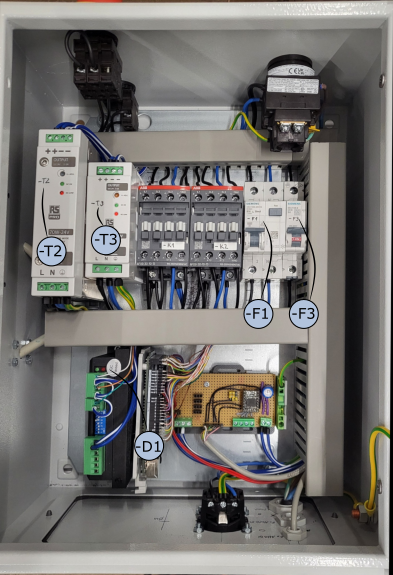
\includegraphics[width=0.6\textwidth]{Abbildungen/Manuel/schrankinnen.png}
    \caption{Schaltschrank}
    \label{fig:schaltschrank}
\end{figure}


Sollte sich das Gerät nicht einschalten lassen kann das an mehreren Problem liegen. Zunächst sollte überprüft werden ob sich der NOT-AUS Schalter in der oberen Stellung befindet. Für den Fall das dies nicht der Fehlergrund ist  muss der Versuchstand jetzt vom Stromnetz getrennt werden. Wie in Abbildung \ref{fig:schaltschrank} kann nun der Schaltschrank geöffnet werden. Zu überprüfen ist nun ob sich die Sicherungen (-F1, -F3) beide in der oberen Stellung stehen. Für weitere Fehlersuche muss der Schrank unter Netzspannung stehen. Wird dies Problemlösung angewandt ist dies mit höchste Vorsicht zu tun. Es dürfen im Schrank nun keine Potentiell bestromten Teile, wie Schrauverbindungen und Kabel, mehr berührt werden. Nach dem Wiedereinschalten  sollten die grünen LED´s an den Netzteilen (-T2, -T3) leuchten, welche deren Funktionsfähigkeit bestätigen. Ebenfalls sollte die grüne LED an -D1 leuchten. Sind alle Lampen auf grün und die Funktionsfähigkeit ist trotzdem nicht gewährleistet liegt wahrscheinlich ein Defekt des Arduinos vor. 
